Die mit dem snort-Flag \inlinecodee{l} generierten Logdateien enthalten nicht die Alarmierungsnachrichten der Konsole, sondern sind Logs des gesamten Traffics. Praktischerweise können diese mit Wireshark geöffnet und nachträglich analysiert werden. Mithilfe der Konsolenausgabe oder eines externen Logs (über Option \inlinecodee{-A fast}) können dann z.B. die Zeiten der Alarme genutzt werden, um die Angriffe in Wireshark ausfindig zu machen. Abb. \ref{fig:wireshark} zeigt einen Ausschnitt der SYN-Flood aus Abschnitt \ref{sec:dos}.

\begin{figure}[H]
\centering
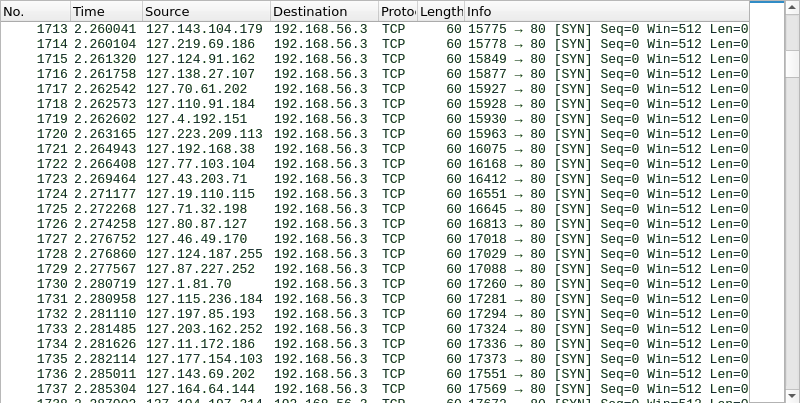
\includegraphics[width=0.7\textwidth]{graphics/attacks/wireshark.png}
\caption{Snort Log in Wireshark}\label{fig:wireshark}
\end{figure}
